% !TEX program = pdflatex
\documentclass[12pt]{article}
\usepackage[reqno]{amsmath}
\usepackage{amssymb,amsthm,graphicx,verbatim,url,verbatim,longtable,vmargin, accents,bbm,times,subfig,dcolumn,booktabs,setspace,soul,latexsym,wasysym,titling,enumitem,longtable,booktabs,xr,caption}
\externaldocument{acc-supp}
\allowdisplaybreaks
% \usepackage{showkeys}

\usepackage[export]{adjustbox}
\usepackage[dvipsnames,usenames]{xcolor}
\definecolor{spot}{rgb}{0.6,0,0}

\usepackage{tikz}\usetikzlibrary{tikzmark,arrows,calc,arrows.meta}
\usepackage[T1]{fontenc}\usepackage[encapsulated]{CJK}\usepackage[utf8]{inputenc}

\newcommand{\icirc}{%
  
\begin{tikzpicture}[baseline=(char.base)]
    \node[shape=circle, fill=lightgray, font=\normalsize, inner sep=1pt, minimum size=1em] (char) {\textcolor{white}{i}};
  \end{tikzpicture}%
}

\usepackage[natbib=true,uniquename=false,minbibnames=1,maxbibnames=99,maxcitenames=1,maxcitenames=3,backend=biber,ibidtracker=false,style=authoryear]{biblatex}
\addbibresource[location=remote]{https://raw.githubusercontent.com/iqss-research/gkbibtex/master/gk.bib}
\addbibresource[location=remote]{https://raw.githubusercontent.com/iqss-research/gkbibtex/master/gkpubs.bib}
\setcounter{biburllcpenalty}{7000}\setcounter{biburlucpenalty}{8000}

\usepackage[all]{xy}
\setpapersize{USletter} \topmargin=0in
\newcolumntype{.}{D{.}{.}{-1}}\newcolumntype{d}[1]{D{.}{.}{#1}}
\graphicspath{{./figs/}}
\renewcommand{\topfraction}{0.85} \renewcommand{\textfraction}{0.1}
\renewcommand{\floatpagefraction}{0.75} % keep < \topfraction
\newcommand{\cntext}[1]{\begin{CJK}{UTF8}{gbsn}#1\end{CJK}}
\newcommand{\btVFill}{\vskip0pt plus 1filll}
\usepackage[titletoc,title]{appendix}
\newtheorem{proposition}{Proposition}
\DeclareMathOperator*{\argmax}{arg\,max}
\DeclareMathOperator*{\argmin}{arg\,min}
\newcommand{\mean}{\operatornamewithlimits{mean}}  
\newcommand{\Cov}{\text{Cov}}
\theoremstyle{definition}
\newcommand{\blind}{0} % 1=blind, 0=not blind
\newcommand{\titl}{Statistical Intuition Without Coding (or Teachers)}
\newcommand{\authr}{Natalie Ayers, Gary King, Zagreb Mukerjee, Dominic Skinnion}

\if1\blind
\title{\titl}
\renewcommand{\authr}{}
\fi
\usepackage[pdftex, bookmarksopen=true, bookmarksnumbered=true,
  pdfstartview=FitH, breaklinks=true, urlbordercolor={0 1 0},
  citebordercolor={0 0 1}, colorlinks=true, citecolor=spot, 
  linkcolor=spot, urlcolor=spot, pdfauthor={\authr},
  pdftitle={\titl}]{hyperref}

\if0\blind
\title{\titl} \thanks{Our thanks to Kenneth Bolen, Aleksandra Conevska, Jamie Druckman, Danny Ebanks, Zach Elkins, Benjamin Goodrich, Connor Jerzak, David Kane, Thad Kousser, Adeline Lo, Thomas Pepinsky, Yotam Shmargad, and an anonymous reviewer through the Alexander and Diviya Magaro Peer Pre-Review Program for helpful comments.}

\author{Natalie Ayers\thanks{Political Science Ph.D.\ student, Institute for Quantitative Social Science, Harvard University, Natalie-Ayers.github.io/home, NatalieAyers@g.harvard.edu}\and Gary King\thanks{Albert J.\ Weatherhead
III University Professor, Institute for Quantitative Social
Science, Harvard University; GaryKing.org, King@Harvard.edu.}\and Zagreb Mukerjee\thanks{Political Science Ph.D.\ student, Yale University, politicalscience.yale.edu/people/Zagreb-Mukerjee, Zagreb.Mukerjee@Yale.edu} \and Dominic Skinnion\thanks{Quantitative Social Science Researcher, Institute for Quantitative Social Science, Harvard University, Dominic\_Skinnion@g.harvard.edu, iq.harvard.edu/people/Dominic-Skinnion}}
\fi

\begin{document}
\maketitle\thispagestyle{empty}\setcounter{page}{0}
\btVFill
\vspace{-2\baselineskip}
\begin{abstract}
  \noindent Two features of quantitative political methodology make teaching and learning especially difficult: (1) Each new concept in probability, statistics, and inference builds on all previous (and sometimes all other relevant) concepts; and (2) motivating substantively oriented students, by teaching these abstract theories simultaneously with the practical details of a statistical programming language (such as R), makes learning each subject harder. We address both problems through a new type of automated teaching tool that helps students see the big theoretical picture and all its separate parts at the same time without having to simultaneously learn to program. This tool, which we make available via \href{https://2k1.iq.harvard.edu}{one click in a web browser}, can be used in a traditional methods class, but is also designed to work without instructor supervision.
  \\
  \newline
  \noindent Words: 2735
\end{abstract}
\btVFill
\clearpage
% \renewcommand{\contentsname}{Contents (page to be removed before publication)}
% \setcounter{tocdepth}{8}\tableofcontents\clearpage
\baselineskip=1.57\baselineskip

\section{Introduction}\label{s:intro}

Most new political science Ph.D.\ students have long since branched off from math and physics and are excited to be able to focus on their substantive interests in government and politics. Yet, upon arrival, many are surprised to learn that their first class will be in quantitative political methodology, and they now need to master a series of highly sophisticated technical concepts, such as the mathematical and statistical theories of uncertainty and inference. Since ``deferral of gratification'' pretty much defines the graduate school experience, most dutifully go along. But then they arrive in class, expecting to be taught these abstract concepts and are told that they must simultaneously learn the practical details of a statistical programming language --- in order to learn (and implement) these abstract concepts, in order to begin to study what they came to graduate school for in the first place.

Abstract statistical theory and practical programming tasks (including, e.g., understanding how maximum likelihood differs from probability theory and fixing that obscure bug in your code on line 57) are, of course, both essential to a career as an empirical political scientist. Although teaching these topics sequentially would be easier and more efficient, it can be demotivating for substantively oriented students. So we try to give them the big picture of how research is justified, designed, and implemented all at the same time, often finding creative ways of using this material to motivate them \citep{williams2022teaching}. Judging from changes in the literature over the last several decades, teachers of political methodology have succeeded spectacularly well in motivating students and making them better political scientists, but even with the best pedagogical strategies our classes do sometimes have the same problems as calculus lectures taught during swimming lessons.

In this paper, we introduce an automated teaching tool designed to help students see the big picture about crucial aspects of statistical theory without having to learn statistical programming (until later) and with minimal distracting ``clutter'' \citep{bailey2019teaching}. It also helps students zoom in on details and out for the big picture, whether or not they already know how to program. This tool, which we call ``2K1-in-Silico: An Interactive Non-Textbook'', is available by clicking on \href{https://2k1.iq.harvard.edu}{2K1.iq.harvard.edu}; no downloads or installations required. (Alternatively, you can download the app from our repository \href{https://github.com/iqss-research/2k1-in-silico}{github.com/iqss-research/2k1-in-silico} and use it off line, or try it in RStudio as a transition to learning to program.) It is designed for self-study, without instructor supervision, although we have used it to complement a class going through each part in depth (by helping to ``teach students to teach themselves''; \citealt{Schleutker2022}).

2K1-in-Silco is named after the class for which it was originally designed, Government 2001, taught by Gary King. This is the first class in the Harvard University political science Ph.D.\ sequence and almost all graduate students in the department take it, along with others from related disciplines and professional schools and nearby universities. 2K1-in-Silico can be used on its own, or by taking Government 2001 at Harvard or online (through the Harvard Extension School).  Most of the materials for this class are also freely available to students and instructors elsewhere for use in their own classes. This includes all the lecture videos, the slides used in the lectures, the syllabus, the readings, and more; see the class website at \href{https://j.mp/G2001}{j.mp/G2001}. The lecture videos can be watched on your own on YouTube at \href{https://bit.ly/gov2001v}{bit.ly/gov2001v} or with others through \href{https://perusall.com}{Perusall.com}, a platform that allows students to help each other by annotating the videos and readings together and through other types of motivating interactions. Instructors teaching their own classes, or groups of students watching together, may create their own free Perusall class account by registering at \href{https://bit.ly/gov2001preg}{bit.ly/gov2001preg}, creating a course, and entering in ``copy code'' \textbf{PCDKPTWZ39}, which pulls in all the videos automatically.

\section{Interconnected Content}

Unlike connections that can often be found among substantive political science research topics, many parts of quantitative political methodology classes are closer to a singular whole and so best studied together. The difficulty is that any digestible, single class- or assignment-sized, piece of this whole is insufficient to convey the big picture. So we march forward, teach each part, and all the while ask students to trust us that the big picture, and fuller understanding, will come into focus over the semester. Because each part is best understood only after understanding all the other parts, students typically refer back to material learned earlier, or sometimes repeat the class or take different classes covering the same material.

In 2K1-in-Silico, we cover these three interrelated topics:
\begin{enumerate}\singlespacing
  \item \emph{Data generation processes}, using probability models;
  \item \emph{Inference}, using likelihood models \citep{King98}; and
  \item \emph{Quantities of interest}, using statistical simulation (see \citealt{KinTomWit00} and Clarify software for R or Stata; see \href{https://GaryKing.org/clarify}{GaryKing.org/clarify}).
\end{enumerate}

Probability enables us to randomly generate data from an assumed mathematical model (e.g., drawing a set of heads and tails from the model of a fair coin flip), whereas the goal of inference is the reverse: learning about features of a given model (such as whether the coin is fair) from a set of observed data (e.g., an observed string of heads and tails from 100 flips of a coin). Quantities of interest are calculated from statistical inferences, based on real data; numerous types of quantities can be computed, such as expected values, predicted values, and probabilities, for use in forecasts, descriptive and counterfactual estimation, or for other purposes.

Probability, inference, and quantities of interest are mostly useful to political scientists with far more sophisticated models than coin flips, of course, allowing for explanatory variables and many possible different dependence structures, distributions, sample spaces, and mathematical formalisms.  2K1-in-Silico presently includes 18 different models, such as linear-normal regression, Poisson and negative binomial count models, exponential duration models, and binary and ordered probit and logit models. (Our software is open source, so anyone can add models if they wish, with some programming of course!)

Understanding one historical period or substantive topic studied by political scientists is usually helpful in studying another, but many topics in political methodology are much more interrelated.  The likelihood theory of inference is defined with probability densities. Computing quantities of interest can be done by simulation or analytic means to learn about the results of likelihood estimation or features of a probability distribution constructed from theory without data. Probability can be studied without the other two topics, but empirical political scientists have little interest in made-up models (or the data they can generate) without any necessary connection to the world we wish to study.

\section{Design Principles}

In building 2K1-in-Silico, we followed several design principles.

First, the main idea is to provide the big picture while enabling students to zoom in and see any details they wish, with nothing omitted, and then zooming back out to understand the context. One of the reasons learning programming is valuable is because it enables us to get a feel for complicated statistical and mathematical objects (such as statistical models) too complicated to fit entirely in one human's working memory, usually by repeatedly running a program, changing its inputs, and seeing what happens to the outputs. We allow users to gain this intuition in 2K1-in-Silico by simple dropdown boxes and slider bars, and watching numerical results and graphics change dynamically and instantly, without any programming.

Second, the documentation for most statistical software packages does not include complete, mathematically precise descriptions of the methods and algorithms implemented, leaving instead only citations to the original scholarly source (sometimes with half-baked equations written in text, like DEPENDENT = alpha + beta1*INDEPENDENT, which usually conveys what is going on only to those who already know). For software users, however, determining whether the method implemented is identical to that in the textbook can then sometimes be difficult. In fact, anyone who writes computer code to implement a method knows that they typically do differ and for good reasons.

For one example, numerical optimization that involves a parameter that can only be positive, say a variance $\sigma^2$, can crash the program if it guesses zero or a negative value on the way to the optimum. Thus, a convenient numerical optimization trick is to reparameterize by defining $\sigma^2=e^\gamma$, and estimating $\gamma$. This is convenient because $\gamma$ can take on any finite value, and so we can optimize the function without constraints and without anything crashing, estimate $\gamma$, and then exponentiate the result. This works well also because $e^{\hat\gamma}$ is the same maximum likelihood estimate as if we had optimized the function directly. That's great but, in fact, the standard errors and full posterior distribution do change with this reparameterization and so replication, and complete understanding, requires knowing how the software is written. Thus, in 2K1-in-Silico, every time a user chooses a model, the full and precise mathematical formulation of the model implemented in the software automatically appears on the page (\LaTeX\ formatted).

Third, to make this tool work as well as possible without instructor intervention, we add next to every object on every page a \icirc\ symbol, enabling the user to request more \underline{i}nformation.  Clicking on any one of those symbols provides the needed information about an equation, dropdown box, statistical model, parameter, covariate, numerical result, dataset, or graphic. The information is presented in a little popup box without causing the user to lose context. In addition to all the \icirc\ symbols, there's a button to ask for a tutorial that will take you on a guided tour of the whole app if desired, which is designed for the most basic users without interfering with those with more advanced skills.

Finally, the program even tries to convey what numerical optimization algorithms do by letting the user guess at parameter values and see what the result looks like in terms of the distance from the maximum likelihood or what the uncertainty estimates look like. At every stage, the data are always available and on the screen, including data that could be generated by a probability model or to be used in making a statistical inference of some kind.

\section{What it does}

Almost by definition, we cannot use the static presentation format of a paper to fully convey what our interactive tool does, and so feel free to click here \href{https://2k1.iq.harvard.edu}{2K1.iq.harvard.edu} and read along in order to see it in action as we explain it. In the app, you will find an overview page with three tabs across the top, corresponding to (1) data generation processes, (2) model inferences, and (3) quantities of inference, intended to be used in this order.  You can start with ``tutorial mode'' or instead skip that and see if the app is as intuitive enough without it, as intended. Either way, for any feature not immediately understandable, merely click on the corresponding \icirc\ to get an in-context, detailed explanation.

Begin by clicking on the data generation process (DGP) tab, and choosing a DGP to explore. The mathematical form of the chosen probability model will instantly appear, along with slider bars for the user to set, indicating the parameter values and number of observations. This is followed by a dataset drawn from the model along with graphic visualizations in a variety of useful formats that automatically change depending on the type of data and model. All options, including the choice of the model, come with defaults, so you do not even need to make any choices if you prefer; however, you will gain intuition if you adjust the inputs and get a feel for how they and the model control the outputs.

To provide a better feel for the app if you have not yet clicked on the link, see Figure \ref{mockscreen} for a snapshot of the app's inference tab.  Along the top row, you can see the tabs that provide context.  Below that is the dataset the user created on the previous (DGP) page.  Although the data was generated by some model of the user's choice there, in the real world we do not know the DGP during inference. Thus, on this page we must choose the assumed distribution for the statistical model, which we can do from the dropdown box (on the top left, with ``Ordered Logit'' showing presently), along with the choice of one or more explanatory variables to include (with their own dropdown boxes, presently showing ``Normal B'' and ``Uniform A,'' with details about them documented in the gray \icirc\ symbol to its right).
\begin{figure}[p]
  %\null
  \vspace*{-1in} 
  \centering
  \begin{adjustbox}{center,valign=c}
    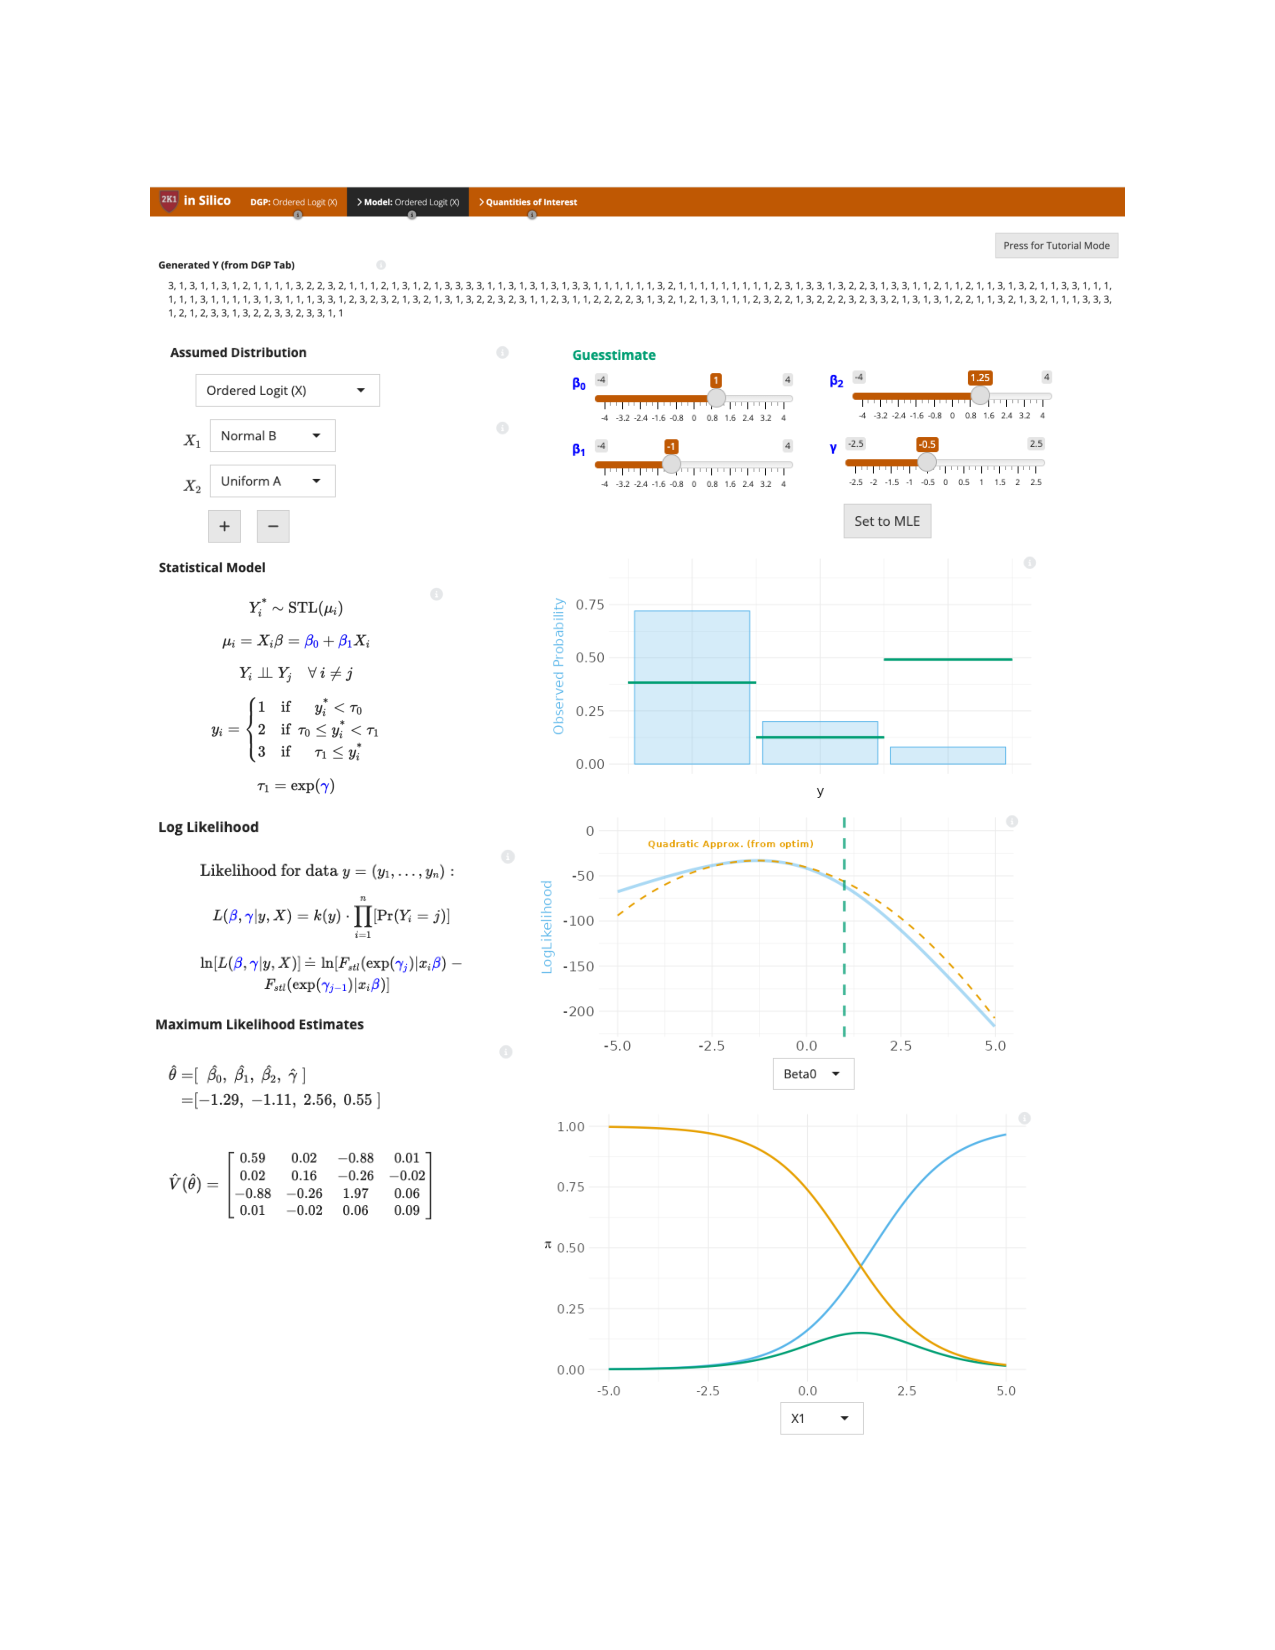
\includegraphics[width=1.5\textwidth]{mockscreen}
  \end{adjustbox}
  \vspace*{\fill} 
  \captionsetup{skip=-95pt}
  \caption{2K1-in-Silico: Model Inference tab (translated to a static figure)}
  \label{mockscreen}
\end{figure}

As soon as you choose an assumed statistical model, the mathematical form of the statistical model appears, followed by the complete mathematical form of the log-likelihood.  At the bottom left, the values of the maximum likelihood estimates and variance matrix appear, but to get a better feel for the maximization process, the slider bars at the top right allow the user to make a ``guesstimate'' of the values of each of the parameters (in blue, corresponding to the values in the math at the left). As the user adjusts these slider bars, the horizontal bars (in green, corresponding to the color of the word ``guesstimate'') in the graph below show how well they fit the empirical histogram of the data. The second graph plots the (profile) log-likelihood function for each parameter (chosen by the dropdown box below it), along with the best quadratic approximation to the log-likelihood which is used for calculating the standard errors.  The dashed green vertical line in this second plot shows how close the user's guesstimate is to the maximum of the log-likelihood function, and will move as you adjust the sliders.  The last graph on this page, which also instantly adjusts based on the slider bars, provides predicted values from the currently chosen model (in this case ordered logit, for each of the three outcome values that sum to one).  If you click on the ``Set to MLE'' button under the slider bars, the bars will adjust automatically to the maximum likelihood estimates, and the user will see the green horizontal bars on the first graph matching the histogram bars exactly, and all the other graphs adjusting automatically.

The last tab enables you to compute any of a variety of quantities of interest.  If you click on the tab, you will see at the top the maximum likelihood estimates and variance matrix from the inference tab. You can choose which quantity interests you and should be calculated.  Given that, the full mathematical details of the estimation and fundamental uncertainty appear, as these are needed for simulating quantities of interest. You can also select values of the explanatory variables via slider bars.  From all this information, 2K1-in-Silico automatically presents a set of colorful graphics to summarize the quantities you chose to compute, along with various types of uncertainty estimates.

At any time, you can go back to the main page to see the big picture, or any of the three tabs.

\section{Concluding remarks}

In addition to trying 2K1-in-Silico or assigning it in class by clicking on \href{https://2k1.iq.harvard.edu}{2K1.iq.harvard.edu}, we hope you will help us extend the tool to a wider variety of models, graphics, methods, and statistical concepts. We could even add additional tabs for understanding data, matching for causal inference, and imputation for missing data, among others.

To do this, you will need to do some programming of course, but we use relatively straightforward R-Shiny technology, as recommended by \citet{Metzger2022}. All the code is open source and freely available at \href{https://github.com/iqss-research/2k1-in-silico}{github.com/iqss-research/2k1-in-silico}.

\singlespace
\printbibliography
\end{document}

